\subsection{SE-16 Consultar periodos de ETS inscritos del alumno}

\begin{figure}[htbp!]
	\begin{center}
		\fbox{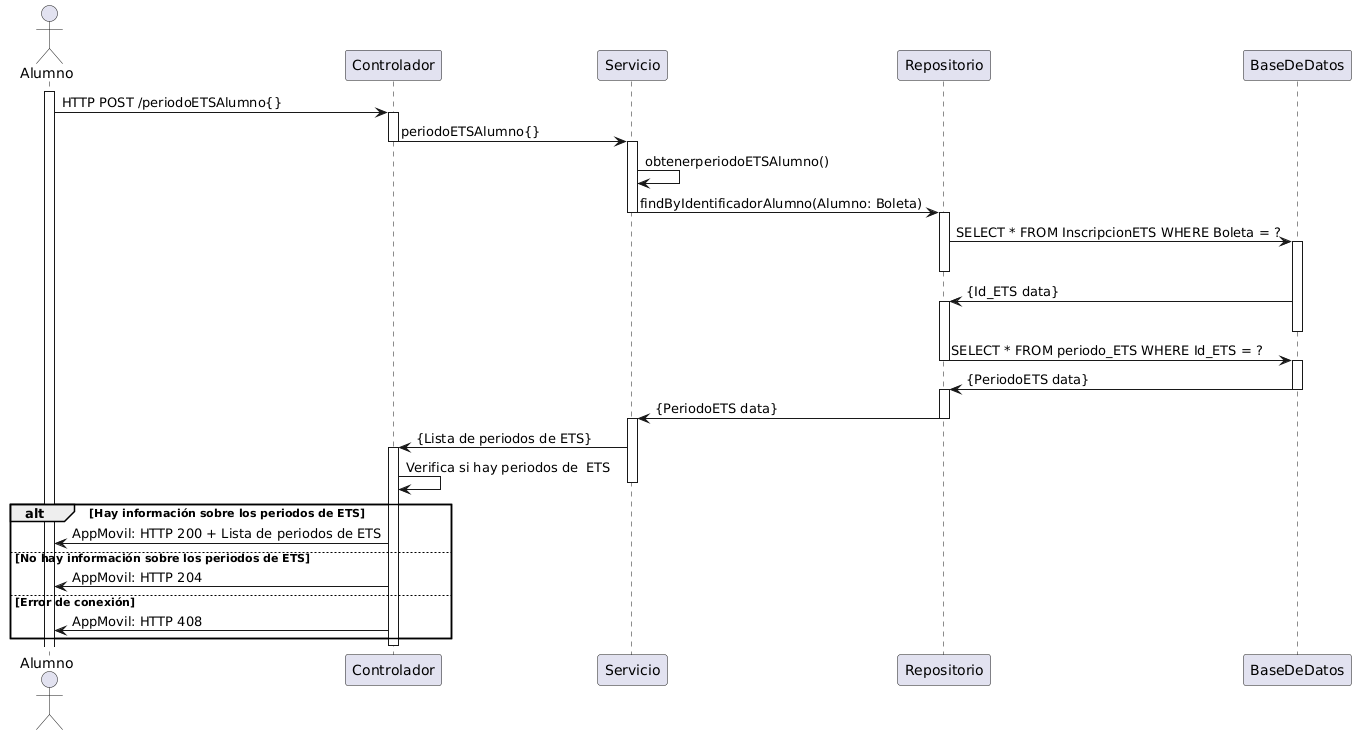
\includegraphics[width=1\textwidth]{Secuencia/CU-16.png}}
		\caption{Diagrama de secuencia del caso de uso número 16 (Consultar periodos de ETS inscritos del alumno).}
		\label{fig:Diagrama de secuencia CU-16}
	\end{center}
\end{figure}

En el diagrama de secuencia \ref{fig:Diagrama de secuencia CU-16} se describe el proceso planeado para el caso de uso \hyperlink{CU-16}{CU-16 Consultar periodos de ETS inscritos del alumno}, mostrando las interacciones que tendrá con la vista, el controlador, el servicio, el repositorio y la base de datos.

\newpage